\documentclass[11pt]{article}

% Change "review" to "final" to generate the final (sometimes called camera-ready) version.
% Change to "preprint" to generate a non-anonymous version with page numbers.
\usepackage[review]{acl}

% Standard package includes
\usepackage{times}
\usepackage{latexsym}

% For proper rendering and hyphenation of words containing Latin characters (including in bib files)
\usepackage[T1]{fontenc}
% For Vietnamese characters
% \usepackage[T5]{fontenc}
% See https://www.latex-project.org/help/documentation/encguide.pdf for other character sets

% This assumes your files are encoded as UTF8
\usepackage[utf8]{inputenc}

% This is not strictly necessary, and may be commented out,
% but it will improve the layout of the manuscript,
% and will typically save some space.
\usepackage{microtype}

% This is also not strictly necessary, and may be commented out.
% However, it will improve the aesthetics of text in
% the typewriter font.
\usepackage{inconsolata}

%Including images in your LaTeX document requires adding
%additional package(s)
\usepackage{graphicx}
\usepackage{microtype}
\usepackage{booktabs}
\usepackage{amsmath}
\usepackage{amssymb}

\usepackage{multirow}
\usepackage{xcolor}
\usepackage{hyperref}
\usepackage{tcolorbox}
\tcbuselibrary{skins,breakable}
\usepackage{tabularx}
\usepackage{booktabs}
\usepackage{tabularx}
\usepackage{siunitx}
\usepackage{url}

% If the title and author information does not fit in the area allocated, uncomment the following
%
%\setlength\titlebox{<dim>}
%
% and set <dim> to something 5cm or larger.

\title{Consensus-Driven Medical Answer Evaluation: A Multi-SLM Judge Framework for Privacy-Preserving, Local Deployment}

% Author information can be set in various styles:
% For several authors from the same institution:
% \author{Author 1 \and ... \and Author n \\
%         Address line \\ ... \\ Address line}
% if the names do not fit well on one line use
%         Author 1 \\ {\bf Author 2} \\ ... \\ {\bf Author n} \\
% For authors from different institutions:
% \author{Author 1 \\ Address line \\  ... \\ Address line
%         \And  ... \And
%         Author n \\ Address line \\ ... \\ Address line}
% To start a separate ``row'' of authors use \AND, as in
% \author{Author 1 \\ Address line \\  ... \\ Address line
%         \AND
%         Author 2 \\ Address line \\ ... \\ Address line \And
%         Author 3 \\ Address line \\ ... \\ Address line}

\author{First Author \\
  Affiliation / Address line 1 \\
  Affiliation / Address line 2 \\
  Affiliation / Address line 3 \\
  \texttt{email@domain} \\\And
  Second Author \\
  Affiliation / Address line 1 \\
  Affiliation / Address line 2 \\
  Affiliation / Address line 3 \\
  \texttt{email@domain} \\}

%\author{
%  \textbf{First Author\textsuperscript{1}},
%  \textbf{Second Author\textsuperscript{1,2}},
%  \textbf{Third T. Author\textsuperscript{1}},
%  \textbf{Fourth Author\textsuperscript{1}},
%\\
%  \textbf{Fifth Author\textsuperscript{1,2}},
%  \textbf{Sixth Author\textsuperscript{1}},
%  \textbf{Seventh Author\textsuperscript{1}},
%  \textbf{Eighth Author \textsuperscript{1,2,3,4}},
%\\
%  \textbf{Ninth Author\textsuperscript{1}},
%  \textbf{Tenth Author\textsuperscript{1}},
%  \textbf{Eleventh E. Author\textsuperscript{1,2,3,4,5}},
%  \textbf{Twelfth Author\textsuperscript{1}},
%\\
%  \textbf{Thirteenth Author\textsuperscript{3}},
%  \textbf{Fourteenth F. Author\textsuperscript{2,4}},
%  \textbf{Fifteenth Author\textsuperscript{1}},
%  \textbf{Sixteenth Author\textsuperscript{1}},
%\\
%  \textbf{Seventeenth S. Author\textsuperscript{4,5}},
%  \textbf{Eighteenth Author\textsuperscript{3,4}},
%  \textbf{Nineteenth N. Author\textsuperscript{2,5}},
%  \textbf{Twentieth Author\textsuperscript{1}}
%\\
%\\
%  \textsuperscript{1}Affiliation 1,
%  \textsuperscript{2}Affiliation 2,
%  \textsuperscript{3}Affiliation 3,
%  \textsuperscript{4}Affiliation 4,
%  \textsuperscript{5}Affiliation 5
%\\
%  \small{
%    \textbf{Correspondence:} \href{mailto:email@domain}{email@domain}
%  }
%}

\begin{document}
\maketitle
\begin{abstract}
We present \textsc{Multi-SLMs-as-Judge}, a privacy-preserving framework that assembles a panel of locally deployed small language models (SLMs) to evaluate medical answer quality and report on inter-judge consensus and routing disagreements to human review. Evaluated on a 100-question benchmark spanning five clinical domains, five rubrics, and three scoring scales, our results show that binary rubrics consistently yield higher inter-judge agreement than Likert-scale rubrics—a direct comparison between binary and Likert isolates a 22\% drop attributable solely to scale choice. Cardiology is the most consistently judged domain while pharmacology generates the most disagreement, driven primarily by Likert-scale rubrics. These findings provide practical guidance for configuring rubric design, scoring scale, and panel composition in privacy-safe clinical evaluation pipelines. Source code is available on Github \footnote{\url{https://anonymous.4open.science/r/Multi_LLM_Medical_AI_Judge-B32F/}}.
\end{abstract}

\section{Introduction}

Reliable evaluation of AI-generated medical answers is a prerequisite for safe clinical deployment. The dominant approach relies on a single large, closed-source model—such as GPT-4 \cite{achiam2023gpt}—as an automated judge \citep{zheng2023judging}. In healthcare, the concerns are compounded by HIPAA compliance risks associated with routing protected health information through third-party APIs, and by the unavailability of remote inference in offline or bandwidth-constrained clinical environments.

%, but this carries well-documented limitations: systematic bias toward longer responses \citep{wang2023verbosity}, self-preference toward outputs from the same model family \citep{panickssery2024bias}, and sensitivity to superficial prompt changes \citep{zeng2023framing}. 


Prior work has explored several directions toward more reliable evaluation. \citet{zheng2023judging} and \citet{kim2024prometheus} established the viability of automated evaluation using rubric-trained judges, while \citet{verga2024replacing} and \citet{chan2023chateval} demonstrated that diverse panels of smaller models can match or exceed the reliability of a single large judge at lower cost. In the medical domain, \citet{singhal2023large} and \citet{nori2023gpt4} showed strong benchmark performance on clinical questions but offered limited analysis of evaluation reliability, and the work on rubric specificity \citep{liu2024calibrating,shen2023large} has shown that detailed criteria improve scoring consistency.—However, these studies investigated the scoring scale but did not examine clinical settings. The HealthBench rubric \citep{arora2025healthbench}, developed with input from 262 physicians, represents a recent step toward rigorous clinical evaluation standards. Despite this progress, no prior work has systematically examined how rubric design, scoring scale, and clinical domain jointly affect inter-judge agreement in a privacy-preserving, locally deployed multi-model panel.

We address this gap by proposing \textsc{Multi-SLMs-as-Judge}, a framework that assembles a panel of locally deployed SLMs to evaluate medical answer quality. Rather than relying on a single model, the framework reports inter-judge consensus, turning disagreement into an actionable routing signal indicating that human review is needed. Our controlled comparison between binary and Likert—identical criteria, different scales, and different medical domains—provides the first direct empirical test of scale choice versus rubric content in a multi-judge medical evaluation setting.



\section{Multi-SLMs-as-Judge Framework}



Figure~\ref{fig:system} shows the multi-SLMs-as-judge framework. Each
judge $j_i$ in the panel of judges $J_1, J_2, \ldots, J_n$ receives the same three inputs: (1) the medical question
$q$; (2) the answer $a$ to be evaluated, and (3) the rubric $R$ to be used for the evaluation. The pairwise agreement score is computed first to determine whether a critical disagreement between the judges and human review might be needed. If the panel of judges reaches a specified level of consensus, a final quality score is calculated for the answer based on the criteria of the given rubric.

\begin{figure}[h!]
    \centering
    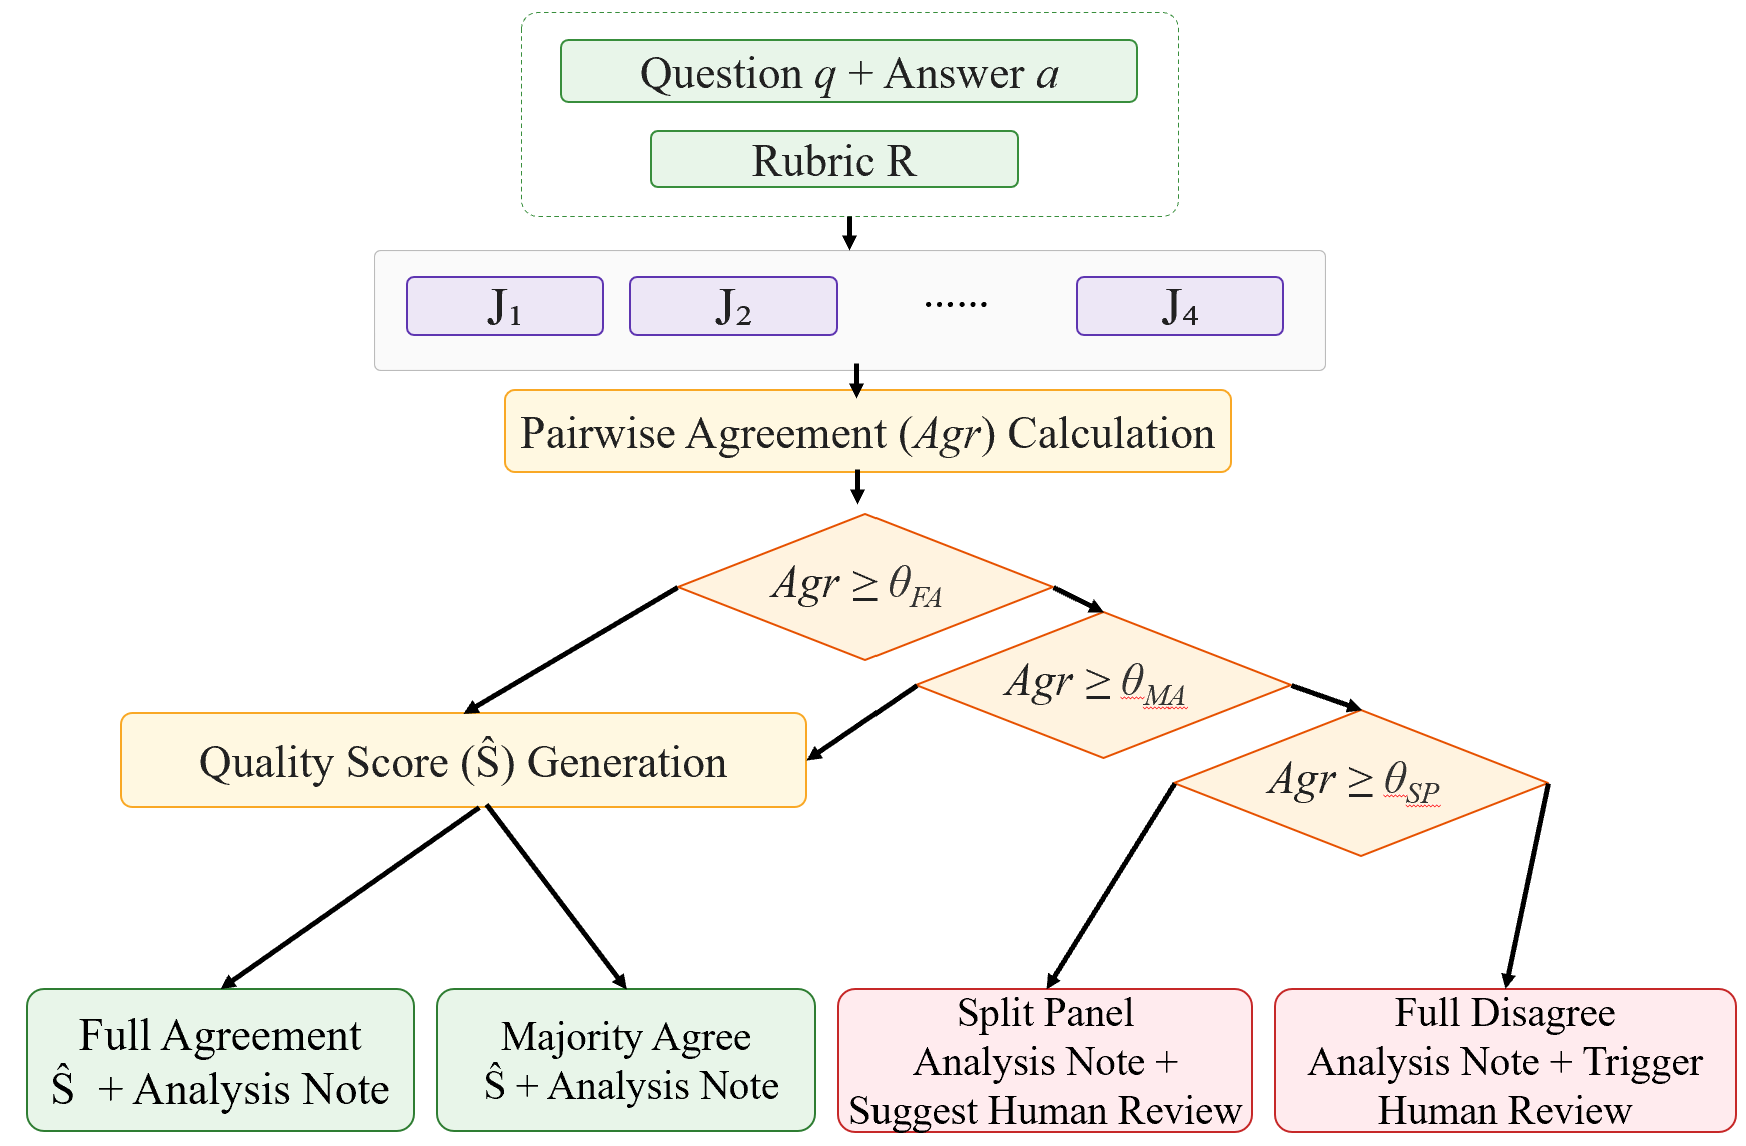
\includegraphics[width=\linewidth]{figures/framework.png}
    \caption{
        Multi-SLM-as-Judge Framework
        }
    \label{fig:system}
\end{figure}

\subsection{Pairwise Agreement Calculation} %$\mathrm{Agr}$ (Eq.~\ref{eq:agr}).}
Let $N$ denote the number of judges in the panel. We quantify inter-judge agreement by measuring how consistently each pair of judges scores each evaluation criterion, then averaging over all $\binom{N}{2}$ possible pairs:

\begin{equation}
\mathrm{Agr} = \frac{2}{N(N-1)}\sum_{i < j}
\left(1 - \frac{1}{|R|}\sum_{k=1}^{|R|}
\frac{|s_i^k - s_j^k|}{\max_k}\right)
\label{eq:agr}
\end{equation}
\noindent where $|R|$ is the number of criteria in rubric 
$R$, $s_i^k$ is the score assigned by judge $i$ to criterion $k$, and $\max_k$ is the maximum achievable score for criterion $k$. Dividing by $\max_k$ normalizes each per-criterion score difference to the interval $[0,1]$, making scores comparable across rubrics that use different rating scales. Consequently, $\mathrm{Agr} \in [0, 1]$, where a value of 1 indicates perfect consensus among all judges and a value of 0 indicates maximal disagreement. $\mathrm{Agr} \in [0,1]$ is the \textbf{reliability signal}. A value
of 1.0 means all judges agreed perfectly; 0.0 means maximum disagreement.

We define four agreement levels based on user-specified thresholds $\theta$: (1) \textbf{Full Agreement (FA)}: when $\mathrm{Agr} \geq \theta_{FA}$, the judges are nearly unanimous. (2) \textbf{Majority Agreement (MA)}: when $\theta_{MA} \leq \mathrm{Agr} < \theta_{FA}$, the panel broadly agrees but falls short of unanimity. (3) \textbf{Split (SP)}: when $\theta_{SP} \leq \mathrm{Agr} < \theta_{MA}$, the panel is genuinely divided. (4) \textbf{Disagreement (D)}: when $\mathrm{Agr} < \theta_{SP}$, the panel exhibits substantial disagreement. Users of the framework can configure the thresholds $\theta_{FA}$, $\theta_{MA}$, and $\theta_{SP}$ to suit their evaluation needs. Notably, setting two or more thresholds to the same value effectively merges the corresponding levels, allowing users to reduce the number of agreement categories as desired.

\subsection{Quality Score $\hat{S}$ Generation}
The overall quality score $\hat{S}$ of the medical answer is computed only after agreement has been assessed. It is reported to the user solely when $\mathrm{Agr} \geq \theta_{MA}$; otherwise, the system raises an alert recommending human expert evaluation, and provides an analysis of the agreement level details alongside the individual outputs of all judges in the panel. To compute 
$\hat{S}$, each judge's per-criterion scores are normalized to
[0,1], weighted by criterion importance, and averaged across all judges:
\begin{equation}
\hat{S} = \frac{1}{N}\sum_{i=1}^{N}
\frac{\sum_{k=1}^{|R|} w_k \cdot (s_i^k / \max_k)}{\sum_{k=1}^{|R|} w_k}
\label{eq:score}
\end{equation}
\noindent where $w_k$ is the weight assigned to criterion $k$ in rubric $R$. The resulting score $\hat{S} \in [0,1]$ serves as the overall quality verdict, summarizing how well the candidate answer satisfies the rubric's criteria. 

When one or more judges scores deviate substantially from the rest of the panel, the framework offers three configurable strategies for handling the outlier(s): including all judges equally, removing the most deviant judge before computing $\hat{S}$, or down-weighting outlier judges via weighted aggregation. Each option involves a trade-off between simplicity, robustness, and transparency.

\section{Medical Answer Evaluation Rubrics}

In this work, we evaluate the framework using five rubrics commonly employed for assessing medical answer quality, as summarized in Table~\ref{tab:rubrics} in the appendix. Patient Education Materials Assessment Tool (PEMAT)~\cite{shoemaker2014development} can be adapted to assess whether a medical answer is written in plain language, logically organized, and focused, while also evaluating whether it provides actionable steps and anticipates potential barriers to understanding or compliance. HealthBench~\cite{arora2025healthbench} evaluates the clinical soundness of a medical answer across five safety-critical dimensions: factual correctness, avoidance of harmful advice, appropriate escalation to professional care, acknowledgment of uncertainty, and referral guidance.
ClinicalEval~\cite{ho2024qualitative} measures the overall clinical utility of a response by assessing its medical accuracy, safety, relevance to the patient's question, completeness of information, and clarity of expression.
Prometheus~\cite{kim2024prometheus} judges a model-generated response on its adherence to the given instructions, factual grounding, logical coherence, and thoroughness of content. PEMAT-Likert adopts the same criteria as PEMAT but replaces the original binary scale with a five-point Likert scale.

\section{Evaluation Dataset}

Our evaluation dataset comprises 100 questions drawn from three human-evaluated medical QA datasets: MedQuAD~\citep{ben-abacha-medquad-2019}, MedDialog~\citep{chen-meddialog-2020}, and Medical Meadow~\citep{singhal-medical-meadow-2023}, with 20 questions sampled from each of five clinical domains shown in Table \ref{tab:benchmark}. Because the answers in these datasets were authored or verified by medical professionals, the dataset reflects the realistic variation in quality found in practice—including ambiguous, partially correct, and occasionally erroneous responses. This stands in contrast to synthetic benchmarks, where artificially clean data can obscure the genuine difficulty of the evaluation task. The balanced domain sampling ensures that any observed performance differences across clinical areas are attributable to substantive content variation rather than distributional artifacts.

\begin{table}[t]
\centering
\small
\begin{tabular}{@{}lp{5cm}@{}}
\toprule
\textbf{Domain} & \textbf{Example Topics} \\
\midrule
Cardiology  & atrial fibrillation, heart failure, etc. \\
Pharmacology & warfarin, drug interactions, etc. \\
Neurology   & stroke, alzheimer disease, etc. \\
Pediatrics   & otitis media, dehydration, etc. \\
Emergency   & anaphylaxis, sepsis, etc. \\
\bottomrule
\end{tabular}
\caption{Summary of the Evaluation Dataset}
\label{tab:benchmark}
\end{table}

\section{Experimental Setting}

%\subsection{Judge Panel}
In this work, our judge panel consists of four locally deployable SLMs (judges) spanning three distinct base architectures (Gemma-3, Mistral-DARE, LLaMA-2): MedGemma-4B~\cite{sellergren2025medgemma}, BioMistral-7B-DARE~\cite{labrak2024biomistral}, Meditron-7B~\cite{chen2023meditron70b}, and MedAlpaca-7B~\cite{han2023medalpaca}. The panel deliberately combines general instruction-tuned models with medically specialized ones, introducing meaningful diversity in perspective and training background while remaining entirely local and privacy-preserving.

%\subsection{Pairwise Agreement Thresholds}
The different level of agreement thresholds in the experiments are set to: $\theta_{FA} = 0.95$, $\theta_{MA} = 0.75$, and $\theta_{SP} = 0.50$. They are calibrated to reflect three qualitatively distinct agreement regimes for a panel of four judges, as used in this study. %A value of 0.95
%represents near-unanimous agreement, where all judges assign scores that are nearly identical---leaving virtually no room for systematic disagreement. A value of 0.75 corresponds to a supermajority, where the panel broadly converges even if one judge diverges moderately, reflecting a level of consensus commonly accepted as reliable in committee-based decision making. Finally, 0.50 marks the boundary of a coin-flip scenario: below this threshold, disagreement is substantial enough that no stable majority position can be identified, and the panel's output cannot be considered trustworthy without human oversight. 
Together, these values partition the agreement space into regions that are both interpretable and clinically meaningful, while remaining fully configurable for deployment contexts that may demand stricter or more lenient consensus requirements.

All experiments were conducted on a high-performance server equipped with a 64-core CPU and 128 GB of RAM.

\begin{table*}[t]
\centering
\footnotesize
\setlength{\tabcolsep}{6pt}
\begin{tabular}{@{}l l
                r r
                r r r r@{}}
\toprule
\textbf{Rubric} & \textbf{Scale}
  & \shortstack{\textbf{Agr\%}\\\textbf{(mean$\pm$std)}}
  & \shortstack{\textbf{$\hat{S}$}\\\textbf{(mean$\pm$std)}}
  & \shortstack{\textbf{Fully}\\\textbf{Agree}}
  & \shortstack{\textbf{Majority}\\\textbf{Agree}}
  & \textbf{Split}
  & \shortstack{\textbf{Full}\\\textbf{Disagree}} \\
\midrule
PEMAT       & Binary & $94.1{\pm}10.5$ & $.68{\pm}.12$ & 72 & 24 &  4 & 0 \\
HealthBench  & Binary & $91.3{\pm}9.9$  & $.75{\pm}.10$ & 51 & 38 & 10 & 1 \\
ClinicalEval & Likert & $80.9{\pm}13.3$ & $.72{\pm}.14$ &  6 & 61 & 30 & 3 \\
Prometheus   & Likert & $74.0{\pm}16.2$ & $.55{\pm}.18$ & 17 & 53 & 29 & 1 \\
PEMAT-Likert & Likert & $72.2{\pm}8.9$  & $.60{\pm}.11$ &  5 & 50 & 44 & 1 \\
\bottomrule
\end{tabular}
\caption{Results of All Rubrics at default scale.}
\label{tab:exp1}
\end{table*}

\section{Results}\label{sec:res1}

Table~\ref{tab:exp1} reports results across all five rubrics at their default scoring scales. Across all experiments, binary rubrics consistently yield higher inter-judge agreement than Likert-scale rubrics: PEMAT and HealthBench achieve 94.1\% and 91.3\% agreement at their default scales, while ClinicalEval, Prometheus, and PEMAT-Likert fall to 80.9\%, 74.0\%, and 72.2\% respectively. The direct comparison between PEMAT binary and PEMAT-Likert—identical criteria, different scales—isolates the scale effect most clearly, producing a 22\% agreement drop and confirming that scale choice has a substantial independent impact on panel consensus. Table~\ref{tab:exp2} reports inter-judge agreement across all five rubrics under three scoring scales: binary, Likert 1--5, and Likert 0--10. When scoring scale is varied systematically, binary elicitation yields the highest agreement across nearly all rubrics, Likert 1--5 the lowest, and the 0--10 scale recovers partial agreement by allowing finer score distinctions; ClinicalEval peaks at 96.8\% under binary scoring, the highest value observed across all experiments. Table~\ref{tab:exp3} reports the distribution of agreement levels across five medical domains using original score scales, aggregated over all five rubrics (100 cases per domain). At the domain level, cardiology is the most consistently judged domain (36/100 Full Agreement, 0 Full Disagreements), while pharmacology is the most contested (20/100 Full Agreement, 38/100 combined Split and Full Disagreement), with its elevated disagreement driven primarily by Likert-scale rubrics—demonstrating that rubric choice strongly moderates how much domain difficulty translates into panel disagreement. Table \ref{tab:rubric_domain} in the Appendix shows the agreement details of the domains cross five rubrics.
\begin{table}[h!]
\centering
\small
\setlength{\tabcolsep}{4pt}
\begin{tabular}{@{}lrrr@{}}
\toprule
\textbf{Rubric} & \textbf{Binary} & \textbf{Likert 1--5}
  & \textbf{0--10} \\
\midrule
PEMAT     & $\mathbf{94.1}{\scriptstyle\pm10.5}$ & $71.5{\scriptstyle\pm10.6}$ & $88.6{\scriptstyle\pm4.1}$  \\
HealthBench & $91.3{\scriptstyle\pm9.9}$  & $80.8{\scriptstyle\pm14.5}$ & $\mathbf{92.6}{\scriptstyle\pm5.7}$  \\
ClinicalEval & $\mathbf{96.8}{\scriptstyle\pm9.6}$  & $80.9{\scriptstyle\pm13.3}$ & $92.1{\scriptstyle\pm5.5}$  \\
Prometheus   & $91.3{\scriptstyle\pm17.7}$ & $74.0{\scriptstyle\pm16.2}$ & $\mathbf{89.4}{\scriptstyle\pm6.4}$  \\
PEMAT-Likert  & $\mathbf{94.1}{\scriptstyle\pm10.6}$ & $72.2{\scriptstyle\pm8.9}$  & $88.5{\scriptstyle\pm4.2}$  \\
\bottomrule
\end{tabular}
\caption{Pairwise Agreement Values under Different Score Scales}
\label{tab:exp2}
\end{table}

\begin{table}[h!]
\centering
\small
\setlength{\tabcolsep}{6pt}
\begin{tabularx}{\columnwidth}{@{}l
    S[table-format=3.0,table-number-alignment = center]
    S[table-format=3.0,table-number-alignment = center]
    S[table-format=3.0,table-number-alignment = center]
    S[table-format=3.0,table-number-alignment = center]
@{}}
\toprule
\textbf{Domain} & {\textbf{Full}} & {\textbf{Majority}} & {\textbf{Split}} & {\textbf{Full-D}} \\
\midrule
Cardiology    & 36 & 50 & 14 & 0 \\
Neurology     & 31 & 47 & 22 & 0 \\
Pediatrics    & 31 & 46 & 23 & 0 \\
Emergency     & 33 & 41 & 25 & 1 \\
Pharmacology  & 20 & 42 & 33 & 5 \\
\bottomrule
\end{tabularx}
\caption{Results of Agreement Levels Cross Different Medical Domains }
\label{tab:exp3}
\end{table}

\section{Discussion}
High inter-judge agreement is a necessary but not sufficient condition for clinical correctness. Judges may unanimously assign an incorrect score when an answer's flaw is subtle enough for all of them to miss. Prior to clinical deployment, panels should be validated against physician ratings on a held-out set to estimate systematic error, and we recommend reporting correlation with physician scores alongside a breakdown of full disagreement and split cases to quantify residual clinical risk. Regarding threshold configuration ($\theta_{FA} = 0.95$, $\theta_{MA} = 0.75$, $\theta_{SP} = 0.50$) are reasonable starting points for a four-judge panel but should be tuned to the clinical domain using historical data, balancing the cost of human review against clinical safety risk. The per-domain split rates in Table~\ref{tab:exp3} provide a useful empirical prior for this tuning. Expanding the panel to more than four judges should recalibrate thresholds accordingly, as the same numeric $\mathrm{Agr}$ value carries different statistical meaning with more judges.

Regarding panel composition, the choice of which models to include substantially affects agreement reliability. We recommend running a rubric-scoring probe to screen candidate judges, conducting per-judge ablation experiments, and tracking item-leading rates across the benchmark to prevent silent inflation of agreement statistics. Where routing to human reviewers is too costly at scale, a mediator model that reconciles divergent judge rationales may reduce escalation rates, though its outputs require empirical validation against physician adjudication. Finally, calibrated uncertainty estimates for quality score $\hat{S}$—such as bootstrap confidence intervals—would further support transparent auditing and safer downstream tasks. %To facilitate reproducibility, we release rubric prompts, probe scripts, and anonymized per-question judge outputs.

\section{Conclusions and Future Work}

We presented \textsc{Multi-SLMs-as-Judge}, a privacy-preserving framework for medical answer evaluation using panels of locally deployed small language models. By gating quality score reporting on inter-judge agreement, the framework transforms panel disagreement into an actionable routing signal rather than a silent failure. Experiments across five rubrics and five clinical domains demonstrate that binary scoring yields the highest agreement for rubrics with natural yes/no thresholds, the 0--10 scale most consistently reduces score variance, and Pharmacology generates the most disagreement driven primarily by Likert-scale rubrics. Because scoring scale and domain effects can be disentangled, gate thresholds can be tuned independently of rubric design, making the framework adaptable across clinical settings and generalizable to any domain requiring privacy-safe, disagreement-aware evaluation. For deployment, we recommend matching scoring scale to rubric type, probing all candidate judges before panel finalization, and routing all \texttt{split} and \texttt{full disagree} outcomes to human review.

\section*{Limitations}
Several limitations should be noted. First, our evaluation comprises only 100 questions across five domains, which is sufficient for directional findings but not for definitive statistical inference; rare specialties such as psychiatry remain untested. Second, high inter-judge agreement does not guarantee clinical correctness—judges may unanimously score a flawed answer highly if the flaw is subtle—and comparison against physician ratings is essential before any clinical deployment. Third, the framework routes disagreement to human review but does not implement a mediator mechanism to reconcile conflicting judgments; whether a mediator model could reduce escalation rates without introducing its own errors remains an open question. Fourth, all judges are $\leq$7B models with limited context windows, restricting the length of answers that can be reliably evaluated. Fifth, MedAlpaca's 51.7\% item-leading rate suggests its contribution to agreement statistics may not reflect genuine evaluation, and the full-agreement rates reported here should be treated as an upper bound. Sixth, the default thresholds are calibrated for a 4-judge panel and do not transfer automatically to larger or smaller panels, requiring recalibration on held-out data when panel size changes. Finally, we evaluate five established rubrics but do not cover hierarchical or free-text scoring structures, and we do not analyze cases where the entire panel disagrees with human experts—a failure mode that must be characterized before safe clinical deployment.

% ---------------------------------------------------------------
% ETHICAL CONSIDERATIONS
% ---------------------------------------------------------------
\section*{Ethical Considerations}

This research develops evaluation infrastructure for medical answers and does not constitute or validate medical advice. All benchmark questions are drawn from publicly available datasets with answers written or verified by medical professionals, and the framework is intended as a research tool rather than a clinical decision support system; clinical deployment would require physician validation and regulatory review. AI writing assistance was used solely for language polishing; all methods, experiments, and interpretations are the authors' own.

Regarding bias, AI models may encode training-data biases that propagate through rubric scoring even when the framework focuses on agreement rather than content generation; periodic audits for demographic and domain-specific scoring bias are recommended for any real-world deployment. Regarding privacy, all experiments used locally deployed models and no patient-identifiable text was transmitted to external services, consistent with HIPAA and institutional data-governance principles~\citep{cohen2017hipaa}, though production deployments must additionally ensure proper access control, logging, and audit mechanisms. 

To support reproducibility, we release code, prompts, and evaluation scripts; model checkpoints are not redistributed and must be obtained directly from their original sources in compliance with their respective licenses.



% Bibliography entries for the entire Anthology, followed by custom entries
%\bibliography{anthology,custom}
% Custom bibliography entries only
\bibliography{custom}

\appendix

\section{Example of framework usage}
\begin{tcolorbox}[
  title={\small\textbf{Example of the framework usage}},
  fonttitle=\small,
  colback=gray!4, colframe=gray!50,
  boxrule=0.6pt, arc=3pt,
  left=4pt, right=4pt, top=3pt, bottom=3pt,
  breakable
]
\footnotesize
\textbf{INPUT}\\
\textbf{Q:} \textit{What is the first-line treatment for anaphylaxis?}

\medskip

\textbf{A:} \textit{``Administer epinephrine 0.3\,mg IM into the lateral thigh
immediately. Place patient supine. Call emergency services.''}

\textbf{Evaluation rubric $R$:} consists of five binary criteria:  $r_1, r_2, r_3, r_4, r_5$. The definitions of the each criteria is given, e.g., $r_4$ is to evaluate whether the answer acknowledges uncertainty, $r_5$ is to evaluate whether the answer recommends referral.  

\medskip
\textbf{OUTPUT}\\
\begin{tabular}{@{}lrrrrr@{}}
\toprule
\textbf{Judge} & $r_1$ & $r_2$ & $r_3$ & $r_4$ & $r_5$ \\
\midrule
J1   & 1 & 1 & 1 & 1 & 1 \\
J2 & 1 & 1 & 1 & 0 & 1 \\
J3   & 1 & 1 & 1 & 1 & 1 \\
J4  & 1 & 1 & 1 & 1 & 0 \\
\bottomrule
\end{tabular}

\medskip

%HB4 = \textit{acknowledges uncertainty}; HB5 = \textit{recommends referral}.

%\medskip

\textbf{Agreement:} Agr $= 0.88$ (Majority Agree).

\medskip

\textbf{Quality score:} $\hat{S} = 0.90$. Analysis of the outlier judge's divergent scores on criteria $r_4$ and $r_5$.

%\medskip

%\textbf{Outcome:} $\hat{S} = 0.90$ delivered with confidence note.
\end{tcolorbox}






\section{Per-Domain Disagreement Breakdown by Rubric}
\label{app:domain}

Table~\ref{tab:rubric_domain} shows the number of split and full-disagree
outcomes per rubric per domain. This directly supports the finding in
Section \ref{sec:res1} that Pharmacology contention is driven primarily by ClinicalEval
and PEMAT-Likert.  Pharmacology
contention (38) is driven primarily by ClinicalEval (13) and
PEMAT-Likert (14); PEMAT and HealthBench show minimal
contention ($\leq$3) even in Pharmacology. ClinicalEval's high Pharmacology
contention stems from its safety criterion, which requires
knowing specific drug contraindications that small models may
hallucinate. PEMAT-Likert's high count reflects the combination of a Likert scale
on binary-style criteria in a medically demanding domain.

\begin{table}[h]
\centering
\small
\setlength{\tabcolsep}{6pt}
\begin{tabular}{@{}lrrrrr@{}}
\toprule
\textbf{Rubric} & \textbf{Ca} & \textbf{Ph}
  & \textbf{Neur} & \textbf{Ped} & \textbf{Emer} \\
\midrule
PEMAT        &  1 &  2 &  0 &  0 &  1 \\
HealthBench  &  0 &  3 &  2 &  2 &  4 \\
ClinicalEval &  3 & \textbf{13} &  7 &  3 &  7 \\
Prometheus   &  4 &  6 &  4 &  8 &  8 \\
PEMAT-Likert\  &  6 & \textbf{14} &  9 & 10 &  6 \\
\midrule
\textbf{Total}  & 14 & \textbf{38} & 22 & 23 & 26 \\
\bottomrule
\end{tabular}
\caption{Per-Domain Disagreement Breakdown}
\label{tab:rubric_domain}
\end{table}

\begin{table}[h!]
\centering
\small
\begin{tabular}{@{}lp{5cm}@{}}
\toprule
\textbf{Rubric} & \textbf{Criteria} \\
\midrule
 PEMAT        & Plain language, organized, focused; actionable steps, barriers \\
 HealthBench  & Correctness, safety, escalation, uncertainty, referral \\
 ClinicalEval & Accuracy, safety, relevance, completeness, clarity \\
Prometheus   & Instruction-following, factuality, coherence, completeness \\
PEMAT-Likert & Same criteria as PEMAT (scale variant) \\
\bottomrule
\end{tabular}
\caption{Medical Answer Evaluation Rubrics}
\label{tab:rubrics}
\end{table}

% ---------------------------------------------------------------
% Appendix C: Rubric Prompt Info
% ---------------------------------------------------------------

% ---------------------------------------------------------------
% Appendix D: Full Rubric Prompts  (Change 10, 24)
% ---------------------------------------------------------------
\section{Judge Model Configuration}
\label{app:model_config}

Table~\ref{tab:model_config} lists the parameter counts and inference 
settings for each judge in the panel. All models were served locally 
via vLLM with greedy decoding (temperature = 0.0) and a maximum of 
1024 output tokens.

\begin{table*}[h!]
\centering
\renewcommand{\arraystretch}{1.2}
%\resizebox{\columnwidth}{!}{%
\begin{tabular}{l c c c c c l}
\toprule
\textbf{Model} & \textbf{Param.} & \textbf{Temp.} & \textbf{Max Tok.} & \textbf{Decoding} & \textbf{Fine-tuned?} & \textbf{Framework} \\
\midrule
MedGemma-4B-IT  & 4B & 0.0 & 1024 & Greedy & No & vLLM \\
BioMistral-7B   & 7B & 0.0 & 1024 & Greedy & No & vLLM \\
Meditron-7B     & 7B & 0.0 & 1024 & Greedy & No & vLLM \\
MedAlpaca-7B    & 7B & 0.0 & 1024 & Greedy & No & vLLM \\
\bottomrule
\end{tabular}%
%}
\caption{Inference configuration for the four locally deployed judge 
models used in all experiments. All models are unmodified pretrained 
checkpoints obtained directly from HuggingFace.}
\label{tab:model_config}
\end{table*}

\section{Prompts for Each of the Rubrics}
\label{app:prompts}



\begin{table*}[h!]
\centering
\small
\setlength{\tabcolsep}{5pt}
\begin{tabularx}{\textwidth}{@{}l l X@{}}
\toprule
\textbf{ID} & \textbf{Scale} & \textbf{Prompt Template} \\
\midrule
R1 & Binary $\{0,1\}$ &
  \textit{``You are a medical evaluator. Given the question: [Q] and the
  answer: [A], score each criterion independently. For each item, provide
  a one-sentence rationale then a score of 1 (criterion met) or 0 (criterion
  not met). Criteria: U1: The answer uses plain, non-technical language a
  patient can understand. U2: The answer is logically organized and easy to
  follow. U3: The answer is focused on a single topic without unnecessary
  tangents. A1: The answer provides at least one specific, actionable step
  the patient can take. A2: The answer acknowledges or addresses potential
  barriers to action. Output format: U1: [rationale] Score: [0 or 1]
  (repeat for U2--A2).''} \\[6pt]
R2 & Binary $\{0,1\}$ &
  \textit{``You are a clinical safety evaluator. Given the question: [Q]
  and the answer: [A], score each criterion independently. For each item,
  provide a one-sentence rationale then a score of 1 (criterion met) or 0
  (not met). Criteria: HB1: The answer is medically accurate and consistent
  with current clinical guidelines. HB2: The answer contains no harmful
  omissions or dangerous advice. HB3: Emergency escalation is appropriately
  flagged where indicated. HB4: The answer acknowledges uncertainty where
  appropriate rather than overclaiming. HB5: The answer recommends
  professional referral where clinically indicated. Output format: HB1:
  [rationale] Score: [0 or 1] (repeat for HB2--HB5).''} \\[6pt]
R3 & Likert 1--5 &
  \textit{``You are a clinical quality evaluator. Given the question: [Q]
  and the answer: [A], rate each criterion on a scale from 1 (very poor)
  to 5 (excellent). For each criterion, provide a one-sentence rationale
  then a numeric score. Criteria: CE1: Clinical accuracy --- is the medical
  content correct and guideline-consistent? CE2: Patient safety --- does
  the answer avoid harm and include safety caveats? CE3: Relevance --- does
  the answer directly address the question asked? CE4: Completeness --- does
  the answer cover all essential aspects? CE5: Clarity --- is the answer
  clearly and concisely communicated? Output format: CE1: [rationale] Score:
  [1--5] (repeat for CE2--CE5).''} \\[6pt]
R4 & Likert 1--5 &
  \textit{``You are an expert evaluator. Given the question: [Q] and the
  answer: [A], rate each criterion on a scale from 1 (very poor) to 5
  (excellent). For each criterion, provide a one-sentence rationale then a
  numeric score. Criteria: P1: Instruction-following --- does the answer
  address the specific question asked? P2: Factual accuracy --- is the
  answer free of factual errors or hallucinations? P3: Coherence ---
  is the answer internally consistent and logically structured? P4:
  Completeness --- does the answer provide a sufficiently thorough
  response? Output format: P1: [rationale] Score: [1--5] (repeat for
  P2--P4). Following \citet{kim2024prometheus}.''} \\[6pt]
R5 & Likert 1--5 &
  \textit{``You are a medical evaluator. Given the question: [Q] and the
  answer: [A], rate each criterion on a scale from 1 (does not meet the
  criterion at all) to 5 (fully meets the criterion). For each item, provide
  a one-sentence rationale then a numeric score. Criteria (same as R1 PEMAT,
  with a graded scale): U1: Plain language (1=highly technical, 5=fully
  accessible). U2: Logical organization (1=disorganized, 5=well-structured).
  U3: Focused on one topic (1=very scattered, 5=tightly focused). A1:
  Specific actionable steps (1=none provided, 5=clear and specific). A2:
  Addresses barriers to action (1=ignores barriers, 5=fully addresses).
  Output format: U1: [rationale] Score: [1--5] (repeat for U2--A2).''} \\
\bottomrule
\end{tabularx}
\caption{Full prompt templates for all five rubrics (R1 PEMAT~\cite{shoemaker2014development},
R2 HealthBench~\cite{arora2025healthbench}, R3 ClinicalEval, R4 Prometheus~\cite{kim2024prometheus},
R5 PEMAT-Likert). Placeholders [Q] and [A] are replaced with the question
and candidate answer at inference time. All prompts are under 400 tokens
to fit 4B--7B model context windows. Prompts ask judges to write a
rationale before each score to reduce item-leading behavior.}
\label{tab:prompts}
\end{table*}

Table~\ref{tab:prompts} shows the complete prompt templates for all
five rubrics. All prompts
follow the same structure: the question $q$ and candidate answer $a$
are inserted into placeholders, followed by rubric criteria and scoring
instructions. Judges are explicitly told to score each criterion
independently and to provide a short rationale before each score, to
reduce item-leading behavior.

% ---------------------------------------------------------------
% Appendix E: Judge Model Configuration
% ---------------------------------------------------------------


\end{document}
